\documentclass[12pt]{article}

\usepackage[a4paper,margin=1in]{geometry}
\usepackage[utf8]{inputenc}
\usepackage{amsmath,amssymb}
\usepackage{graphicx}
\usepackage{cite}
\usepackage{xcolor}
\usepackage{listings}
\usepackage{caption}
\usepackage{subcaption}
\usepackage{float}
\usepackage{hyperref}
\hypersetup{
	colorlinks=true,
	linkcolor=blue,
	citecolor=blue,
	urlcolor=blue,
}
\definecolor{codebg}{RGB}{248,248,248}
\definecolor{codekeyword}{RGB}{0,92,197}
\definecolor{codecomment}{RGB}{106,153,85}
\definecolor{codestring}{RGB}{196,26,22}
\definecolor{codenumber}{RGB}{128,128,128}
\lstset{
	backgroundcolor=\color{codebg},
	basicstyle=\ttfamily\small,
	breaklines=true,
	frame=single,
	language=Python,
	numbers=left,
	numberstyle=\tiny\color{codenumber},
	keywordstyle=\color{codekeyword}\bfseries,
	commentstyle=\color{codecomment}\itshape,
	stringstyle=\color{codestring},
	showtabs=false,
	showstringspaces=false,
	tabsize=4,
}

\title{Neural Approaches to Code Generation: From Natural Language Understanding to Structured Program Synthesis}
\author{Md Mubin Islam Alif}
\date{\today}

\begin{document}

\maketitle

\begin{abstract}
Code generation nowadays is producing executable code from natural language descriptions. This paper explores the latest neural approaches to code generation, focusing on how models understand natural language and synthesize structured programs. This paper is reviewing three papers: CodeT5~\cite{DBLP:journals/corr/abs-2109-00859}, InCoder~\cite{fried2023incodergenerativemodelcode}, and StructCoder~\cite{10.1145/3636430}. Here I am discussing the methodologies, strengths, and limitations of each approach, and how they contribute to advancing the state of the art in code generation. Here CodeT5 presents an identifier-aware encoder-decoder architecture for code understanding and generation~\cite{DBLP:journals/corr/abs-2109-00859}. InCoder focuses on code infilling and synthesis through a generative modeling approach~\cite{fried2023incodergenerativemodelcode}. StructCoder adds structure awareness to improve generation quality on code translation and text-to-code tasks~\cite{10.1145/3636430}.
\end{abstract}

\section{Introduction}
The idea of code generation from natural language has been fascinating researchers for a long time. With the progressive work in deep learning and some transformer-based models, we have seen significant advancements in this area. The ability of machines to understand natural language and generate structured code has the potential to revolutionize software development. But the issue has been that while models can generate code, they often struggle with understanding the gist of programming logic and structure, which eventually leads to code that may be syntactically correct but semantically flawed. But sometimes even syntactical correctness is flawed as the models are not even aware of the identifiers and structure of the code. This is where models like CodeT5, InCoder, and StructCoder come into play, each addressing different aspects of the code generation problem.

These three models have introduced three different mechanisms to improve code generation. CodeT5 is built on the T5 architecture which is a transformer-based model that has been adapted for code understanding and generation. But on top of it, CodeT5 incorporated the idea of being identifier-aware, which means that it can better understand the role of identifiers in code, which is crucial for generating meaningful and functional code. InCoder, on the other hand, greatly focuses on code infilling and synthesis. It uses a generative modeling approach which allows it to fill in missing parts of code and generate new code based on the context provided. This is particularly useful for tasks like code completion and code repair. StructCoder went one more step beyond. It added structure awareness to the model, which means that it can better understand the hierarchical and logical structure of the code. These all three models have shown significant improvements in code generation, but they also have their own limitations.

\section{Literature Review}
\subsection{Background and Problem Formulation}
When we talk about code generation, we are essentially meaning two things: (1) \textit{natural language to code} (NL-to-PL) generation, where the model takes a natural language description and generates code. (2) \textit{code to natural language} (PL-to-NL) generation, where the model takes code and generates a natural language description of what the code does. Both of these tasks are important for different aspects. The former is crucial for automating software development, where developers can simply describe what they want in natural language and the model can interpret that and generate the corresponding code. The latter is important for code documentation and understanding, where developers use natural language to explain what code does. It helps in understanding the codebase and maintaining the codebase effectively. It eventually helps in documentation and code review processes. But both tasks need to understand the intent, generate syntactically correct code, and also generate semantically meaningful code. This is where the challenge lies.
Early code generation focused on neural networks that were trained on large code corpora. But the transformer's self-attention mechanism proved to be much more of a game changer for capturing long-range dependencies in code~\cite{vaswani2023attentionneed}. Pre-training on large unlabeled code corpora (e.g., GitHub) became standard, with objectives such as masked language modeling (MLM), denoising autoencoding (DAE), and replaced token detection (RTD).
\subsection{Key Challenges in Neural Code Generation}
Based on the three papers, we can identify several key challenges in natural code generation.
\begin{itemize}
	\item \textbf{Understanding Natural Language}: One of the big challenges out there is that the model needs the ability to understand natural language descriptions accurately. But the thing is that natural language can be ambiguous. The model needs to understand the intent behind the natural language description.
	\item \textbf{Identifier Semantics}: As highlighted by CodeT5, understanding identifiers and their semantics is crucial for generating meaningful code. Identifiers are the names given to variables, functions, classes, etc. If the model does not understand the semantics of identifiers, it may generate code that might be syntactically correct but semantically meaningless. 
	\item \textbf{Structural Awareness}: From StructCoder~\cite{10.1145/3636430}, we can see that if we understand the structure of the code, then we can generate better code. Code has a hierarchical structure, and understanding this structure is crucial for generating code that is not only syntactically correct but also semantically meaningful. Here the models need to understand how the different parts of the code relate to each other and how they fit together.
	\item \textbf{Infilling and Editing}: InCoder~\cite{fried2023incodergenerativemodelcode} focuses on code infilling and synthesis. This is a huge challenge as the models need to be able to fill in missing parts of code and generate new code based on the context provided. This feature is particularly useful for tasks like code completion and code repair, but it requires the model to have a deep understanding of the code context and also the ability to generate code that fits well within that existing context.
	\item \textbf{Bidirectional Alignment}: Another challenge is bidirectional alignment. This means that the model should be well aligned in both directions: from natural language to code and from code to natural language.
\end{itemize}
\subsection{Related Pre-trained Models for Code}
	Several pre-trained models have been proposed other than the three focal papers I would be discussing. CodeBERT~\cite{feng2020codebertpretrainedmodelprogramming} is an encoder-only model trained with MLM and replaced token detection on NL-PL pairs. GraphCodeBERT~\cite{guo2021graphcodebertpretrainingcoderepresentations} incorporates data flow graphs into the encoder. PLBART~\cite{ahmad2021unifiedpretrainingprogramunderstanding} is an encoder-decoder model pre-trained with denoising autoencoding on code and natural language. Even though these models are somewhat effective, the decoder here lacks awareness of code structure.
\section{Methodologies}
\subsection{CodeT5: Identifier-aware Encoder-Decoder Model}
CodeT5 is built on the T5 architecture which is a transformer-based model which has been used for various natural language processing tasks  (e.g, Code Understanding, code generation, code translation, etc.). Firstly if I want to summarize the architecture of CodeT5 in two words then it would be Explicit and Focused understanding. CodeT5 is designed to be identifier-aware, which means that it understands the role of identifiers in code generally in a better way than other compatriots.
For natural language processing tasks, there were several powerful models like BERT, GPT, T5, etc. These models were pre-trained on large corpora of text data and then for smaller tasks they were fine tuned. As a result, even for less amount of data, there was good performance. So researchers were thinking that if we could do the same thing for code, then we could also get good performance for code generation and code understanding tasks. So they were trying to apply NLP models. Example:
\begin{lstlisting}
def add(a, b):
    return a + b
\end{lstlisting}
Then the model can learn that it is a function and then perform addition. But the main problem occurred that the model seemed to be one-sided. Some models like BERT were just better for understanding the code, and some models acted like just decoders (e.g. GPT), which were just better for generating code. But we wanted both generation and understanding. So these single-type models are not enough for us. The second problem was that the previous models were just taking the words as a sequence. But in reality, code is much more structured. Example:
\begin{lstlisting}
binarySearch(arr.left,right,x)
\end{lstlisting}
Here the binary search is a function name and those arr, left, right, x are variables. So in CodeT5, they proposed a unified model where the encoder and decoder are trained together. And the main idea around CodeT5 is:
\begin{itemize}
	\item \textbf{Identifier-aware Learning}: The model would understand which one is an identifier and which one is not. Example:
	\begin{lstlisting}
def binarySearch(arr.left,right,x)
	\end{lstlisting}
	Here the model would understand that binarySearch is a function name and arr is an array and left, right are position variables. Understanding these meanings is necessary.
	\item \textbf{Trained using Masked Language Modeling}: 
	It means that when training, some identifiers are masked and the model is trained to predict those masked identifiers. This helps the model to learn the semantics of identifiers and how they relate to each other in the code.
	\item \textbf{Using code and comment together}: For a lot of code there are comments. Example:
	\begin{lstlisting}
# increment value
def inc(x):
	return x + 1
	\end{lstlisting}
	Here the model would learn comment-to-code relation. So if we give the input phrase ``increment value'', then the model would understand that it needs to generate a function that increments a value. The vice versa is also true.
	\item \textbf{Dual learning}: The model is trained in a dual learning manner, which means it is trained for NL-to-PL generation and PL-to-NL generation at the same time.
\end{itemize}
The previous models would see the code as a sequence of tokens.
Code snippet:
\begin{lstlisting}
def add(a, b):
	return a + b
\end{lstlisting}
Here the previous models would just see it as a sequence of tokens such as \texttt{def}, \texttt{add}, \texttt{a}, and \texttt{b}, along with punctuation symbols. But the problem around that was that all models being treated as the same. But in code all tokens are not equal. Here \texttt{def} is a keyword and \texttt{add}, \texttt{a}, and \texttt{b} are identifiers. The identifiers being so much important are because with those developer gives their code a meaning and other people then would understand what the code is trying to interpret and deliver.

The issues of previous models are:
\begin{itemize}
	\item \textbf{Identifier Recognition Issue}: Previously, models would not recognize function names and array names. They would just see them as some random words.
	\item \textbf{Lost of Meaning}: Code snippet:
	\begin{lstlisting}
def binarySearch(arr.left,right,x)
	\end{lstlisting}
	Before, the model would think that binarySearch here is just a token. But in reality, it is a search algorithm, which they would not understand.
	\item \textbf{Problem in Masking}: Code Snippet:
	\begin{lstlisting}
def Mask(arr, left, right, x):
	\end{lstlisting}
	The previous models would just guess randomly as they would not know that they are identifiers.
\end{itemize}
Then in CodeT5:
\begin{itemize}
	\item \textbf{Detecting Identifier}: Here it is explicitly trained to detect identifiers. So it would understand that binarySearch is a function name and arr is an array and left, right are position variables. Understanding these meanings is necessary.
	\item \textbf{Specialized Training}:
		\begin{itemize}
			\item \textbf{Task 1: Identifier Tagging}:
			\begin{itemize}
				\item \texttt{arr} $\rightarrow$ 1 (identifier)
				\item \texttt{def} $\rightarrow$ 0 (not identifier)
			\end{itemize}
			\item \textbf{Task 2: Masked Identifier Prediction}:
			Code Snippet:
			\begin{lstlisting}
def Mask(arr, left, right, x):
			\end{lstlisting}
			The model is trained to predict masked identifiers. So it would learn the semantics of identifiers and how they relate to each other in the code. So this model would have to recover binarySearch from the masked code snippet.
		\end{itemize}
\end{itemize}
The reason behind CodeT5 using T5 architecture is that using one model here, code summarization, generation, translation, and defect detection can be done. So it is a unified model for all code related tasks. The main idea here is that the encoder and decoder are trained together. So the model can learn to understand the code and also generate the code at the same time. T5 uses an Encoder-Decoder structure. There, the encoder understands the input (code/text) and the decoder generates the output. But in CodeT5, it not only understands the code but also generates the code and understands the identifiers. So CodeT5 added identifier awareness and special training objectives to the T5 architecture to improve code understanding and generation performance.
The main ideas of pretraining in CodeT5 are:
\begin{itemize}
	\item \textbf{Identifier-aware Masked Span Prediction}: Example 1:
	\begin{lstlisting}
def add(a, b):
	return a + b
	\end{lstlisting}
	After Masking the code snippet:
	\begin{lstlisting}
def [MASK](a, b):
	return a + b
	\end{lstlisting}
	Here identifiers are masked more and more as the identifiers are meaningful and important. 
	Example 2:
	\begin{lstlisting}
def calculateTotal(price):
	\end{lstlisting}
	After Masking the code snippet:
	\begin{lstlisting}
def <mask>(<mask>):
	\end{lstlisting}

	Here the model would guess calculateTotal and price. So the model gets compelled to learn the context and semantics.

	\item \textbf{Bimodal Dual Generation}:
	Here the model is trained in two ways:
	\begin{itemize}
		\item \textbf{(A) Natural language to code generation}
		\textbf{Input (Example):}
		\begin{lstlisting}
Add two numbers
		\end{lstlisting}
		\textbf{Output:}
		\begin{lstlisting}
def add(a, b):
    return a + b
		\end{lstlisting}

		\item \textbf{(B) Code to natural language generation}
		\textbf{Input (Example):}
		\begin{lstlisting}
def add(a, b):
    return a + b
		\end{lstlisting}
		\textbf{Output:}
		\begin{lstlisting}
Add two numbers
		\end{lstlisting}
	\end{itemize}
	As a result, the model understands the code and also it can write the code better.
	\item \textbf{Multi-task Learning}:
	Here all tasks are trained together. As a result, the model becomes much more versatile and can perform all the tasks using one model.


\end{itemize}
\subsubsection{Model Architecture Overview}
The architecture of CodeT5 is based on the T5 model, which is an encoder-decoder transformer architecture. The encoder takes the input and decoder generates the output. The main novelty here is that the model is trained to be identifier-aware. 

\begin{figure}[H]
\centering
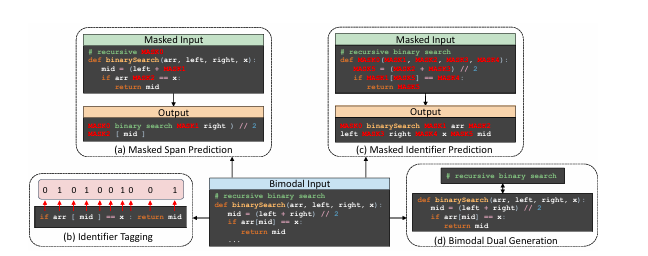
\includegraphics[width=0.85\textwidth]{codeT5demo.png}
\caption{Pre-training tasks of CodeT5. We first alternately train span prediction, identifier prediction, and identifier tagging on both unimodal and bimodal data, and then leverage the bimodal data for dual generation training~\cite{DBLP:journals/corr/abs-2109-00859}}\label{fig:codet5_pretraining}
\end{figure}
The important thing here is its Masked Span Prediction. Here the identifiers are masked more frequently than non-identifiers. Here bimodal dual generation is also important. Here the model is trained to generate code from natural language and also to generate natural language from code. This dual training helps the model to understand the code better and also to generate better code.

\subsection{InCoder: Generative Model for Code Infilling and Synthesis}

InCoder mainly introduces a generative modeling approach for code infilling and synthesis. The main idea is that the model can fill in missing parts of code and generate new code based on the context provided. For previous models like GPT/Codex, it would just generate code from left to right. But in InCoder, it can generate code in any direction. Now I will discuss the training idea here:
Suppose the original code snippet is:
	\begin{lstlisting}
def add(a, b):
	return a + b
\end{lstlisting}
\begin{itemize}
	\item \textbf{Step 1: Masking a little portion}:
	\begin{lstlisting}
def add(a, b):
	<MASK>
	\end{lstlisting}
	\item \textbf{Step 2: Taking the hidden part at last}:
	\begin{lstlisting}
def add(a, b):
	<MASK>
<MASK> return a + b <EOM>
	\end{lstlisting}
	Now the model is trained here to predict the sequence. As a result, the model learns that there is code at the top, at the bottom there is context, and then what would be the code in the middle. So it learns to fill in the missing part. It can be generalized as such that Left context + Right context $\rightarrow$ Missing part. So the model learns to generate code based on the context provided. This is bidirectional context and it is very useful for code infilling and synthesis. 
	
\end{itemize} 
Inference in Real:
Suppose the code snippet is:
\begin{lstlisting}
def square(x):
	<MASK>
\end{lstlisting}
Now we give it to the model. Then the model can predict the missing part. And the model gives the output as:
\begin{lstlisting}
	return x * x
\end{lstlisting}

Real use cases according to the paper~\cite{fried2023incodergenerativemodelcode} are:
\begin{itemize}
	\item \textbf{Variable Rename}:
	Before:
	\begin{lstlisting}
x = 4
y = x + 2

	\end{lstlisting}
	Masked code:
	\begin{lstlisting}
<MASK> = 4
y = <MASK> + 2
	\end{lstlisting}
	Model:
	\begin{lstlisting}
num = 4
y = num + 2
	\end{lstlisting}
	\item \textbf{Docstring Generation}:
	\begin{lstlisting}
def add(a, b):
	return a + b
	\end{lstlisting}
	Masked code:
	\begin{lstlisting}
def add(a, b):
	"""<MASK>"""
	return a + b

	\end{lstlisting}
	\item \textbf{Type Prediction}:
	\begin{lstlisting}
def add(a: int, b: int) -> <MASK>:
	return a + b
	\end{lstlisting}
	The output would be:
	\begin{lstlisting}
	int
	\end{lstlisting}
	\item \textbf{Missing Code Fill}:
	\begin{lstlisting}
for i in range(n):
	<MASK>
	\end{lstlisting}
	The output would be:
	\begin{lstlisting}
print(i)
	\end{lstlisting}

\end{itemize}
The reason this model is this much powerful is that it can understand the context from both sides. So then it is able to generate code that fits very well within the existing context. For old models, it was:
only Left $\rightarrow$ Right.
But in InCoder, it is left context + right context $\rightarrow$ Middle Fill. So it is much more powerful and useful for code infilling and synthesis.
The intuitive idea here is that suppose we are solving a problem and writing code:
 \begin{lstlisting}
	for(int i = 0; i < n; i++){
		//something missing
	}
 \end{lstlisting}
InCoder basically sees the problem, loop, and context and then tries to guess what should be inside. 






\section{Draft Structure}
This section can be replaced with the actual content of the paper. A typical technical paper in this format can include a problem statement, methodology, experiments, results, and discussion. Keeping the layout in one column makes it easier to write, review, and annotate while preserving IEEE-style citations.

\section{Conclusion}
The document is now set up as a single-column LaTeX file with IEEE numeric references. You can expand each section as needed without changing the layout or citation style.

\bibliographystyle{IEEEtran}
\bibliography{references}

\end{document}



